% Graphic for TeX using PGF
% Title: /home/martin/Downloads/trådar.dia
% Creator: Dia v0.97.2
% CreationDate: Mon Oct  6 14:56:04 2014
% For: martin
% \usepackage{tikz}
% The following commands are not supported in PSTricks at present
% We define them conditionally, so when they are implemented,
% this pgf file will use them.
\ifx\du\undefined
  \newlength{\du}
\fi
\setlength{\du}{15\unitlength}
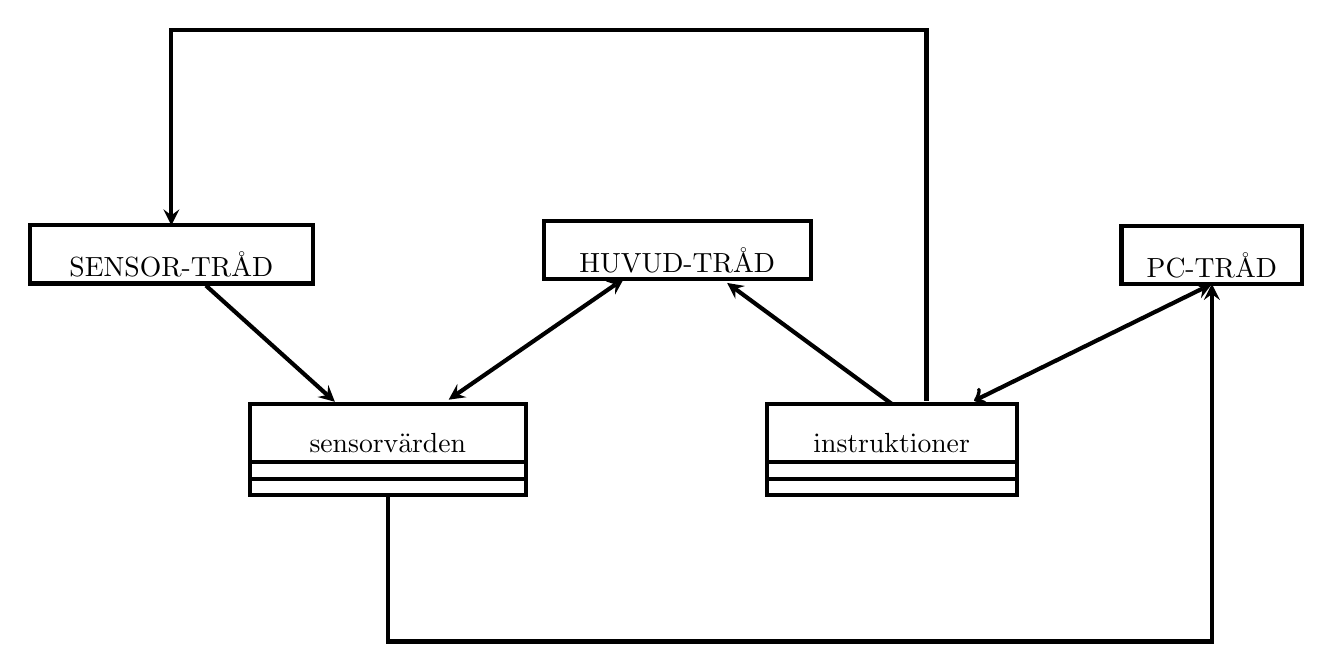
\begin{tikzpicture}
\pgftransformxscale{1.000000}
\pgftransformyscale{-1.000000}
\definecolor{dialinecolor}{rgb}{0.000000, 0.000000, 0.000000}
\pgfsetstrokecolor{dialinecolor}
\definecolor{dialinecolor}{rgb}{1.000000, 1.000000, 1.000000}
\pgfsetfillcolor{dialinecolor}
\pgfsetlinewidth{0.100000\du}
\pgfsetdash{}{0pt}
\definecolor{dialinecolor}{rgb}{1.000000, 1.000000, 1.000000}
\pgfsetfillcolor{dialinecolor}
\fill (83.362742\du,-37.782161\du)--(83.362742\du,-36.382161\du)--(89.792742\du,-36.382161\du)--(89.792742\du,-37.782161\du)--cycle;
\definecolor{dialinecolor}{rgb}{0.000000, 0.000000, 0.000000}
\pgfsetstrokecolor{dialinecolor}
\draw (83.362742\du,-37.782161\du)--(83.362742\du,-36.382161\du)--(89.792742\du,-36.382161\du)--(89.792742\du,-37.782161\du)--cycle;
% setfont left to latex
\definecolor{dialinecolor}{rgb}{0.000000, 0.000000, 0.000000}
\pgfsetstrokecolor{dialinecolor}
\node at (86.577742\du,-36.832161\du){HUVUD-TRÅD};
\pgfsetlinewidth{0.100000\du}
\pgfsetdash{}{0pt}
\definecolor{dialinecolor}{rgb}{1.000000, 1.000000, 1.000000}
\pgfsetfillcolor{dialinecolor}
\fill (70.982742\du,-37.669161\du)--(70.982742\du,-36.269161\du)--(77.805242\du,-36.269161\du)--(77.805242\du,-37.669161\du)--cycle;
\definecolor{dialinecolor}{rgb}{0.000000, 0.000000, 0.000000}
\pgfsetstrokecolor{dialinecolor}
\draw (70.982742\du,-37.669161\du)--(70.982742\du,-36.269161\du)--(77.805242\du,-36.269161\du)--(77.805242\du,-37.669161\du)--cycle;
% setfont left to latex
\definecolor{dialinecolor}{rgb}{0.000000, 0.000000, 0.000000}
\pgfsetstrokecolor{dialinecolor}
\node at (74.393992\du,-36.719161\du){SENSOR-TRÅD};
\pgfsetlinewidth{0.100000\du}
\pgfsetdash{}{0pt}
\definecolor{dialinecolor}{rgb}{1.000000, 1.000000, 1.000000}
\pgfsetfillcolor{dialinecolor}
\fill (76.282742\du,-33.369161\du)--(76.282742\du,-31.969161\du)--(82.932742\du,-31.969161\du)--(82.932742\du,-33.369161\du)--cycle;
\definecolor{dialinecolor}{rgb}{0.000000, 0.000000, 0.000000}
\pgfsetstrokecolor{dialinecolor}
\draw (76.282742\du,-33.369161\du)--(76.282742\du,-31.969161\du)--(82.932742\du,-31.969161\du)--(82.932742\du,-33.369161\du)--cycle;
% setfont left to latex
\definecolor{dialinecolor}{rgb}{0.000000, 0.000000, 0.000000}
\pgfsetstrokecolor{dialinecolor}
\node at (79.607742\du,-32.419161\du){sensorvärden};
\definecolor{dialinecolor}{rgb}{1.000000, 1.000000, 1.000000}
\pgfsetfillcolor{dialinecolor}
\fill (76.282742\du,-31.969161\du)--(76.282742\du,-31.569161\du)--(82.932742\du,-31.569161\du)--(82.932742\du,-31.969161\du)--cycle;
\definecolor{dialinecolor}{rgb}{0.000000, 0.000000, 0.000000}
\pgfsetstrokecolor{dialinecolor}
\draw (76.282742\du,-31.969161\du)--(76.282742\du,-31.569161\du)--(82.932742\du,-31.569161\du)--(82.932742\du,-31.969161\du)--cycle;
\definecolor{dialinecolor}{rgb}{1.000000, 1.000000, 1.000000}
\pgfsetfillcolor{dialinecolor}
\fill (76.282742\du,-31.569161\du)--(76.282742\du,-31.169161\du)--(82.932742\du,-31.169161\du)--(82.932742\du,-31.569161\du)--cycle;
\definecolor{dialinecolor}{rgb}{0.000000, 0.000000, 0.000000}
\pgfsetstrokecolor{dialinecolor}
\draw (76.282742\du,-31.569161\du)--(76.282742\du,-31.169161\du)--(82.932742\du,-31.169161\du)--(82.932742\du,-31.569161\du)--cycle;
\pgfsetlinewidth{0.100000\du}
\pgfsetdash{}{0pt}
\definecolor{dialinecolor}{rgb}{1.000000, 1.000000, 1.000000}
\pgfsetfillcolor{dialinecolor}
\fill (88.732742\du,-33.369161\du)--(88.732742\du,-31.969161\du)--(94.760242\du,-31.969161\du)--(94.760242\du,-33.369161\du)--cycle;
\definecolor{dialinecolor}{rgb}{0.000000, 0.000000, 0.000000}
\pgfsetstrokecolor{dialinecolor}
\draw (88.732742\du,-33.369161\du)--(88.732742\du,-31.969161\du)--(94.760242\du,-31.969161\du)--(94.760242\du,-33.369161\du)--cycle;
% setfont left to latex
\definecolor{dialinecolor}{rgb}{0.000000, 0.000000, 0.000000}
\pgfsetstrokecolor{dialinecolor}
\node at (91.746492\du,-32.419161\du){instruktioner};
\definecolor{dialinecolor}{rgb}{1.000000, 1.000000, 1.000000}
\pgfsetfillcolor{dialinecolor}
\fill (88.732742\du,-31.969161\du)--(88.732742\du,-31.569161\du)--(94.760242\du,-31.569161\du)--(94.760242\du,-31.969161\du)--cycle;
\definecolor{dialinecolor}{rgb}{0.000000, 0.000000, 0.000000}
\pgfsetstrokecolor{dialinecolor}
\draw (88.732742\du,-31.969161\du)--(88.732742\du,-31.569161\du)--(94.760242\du,-31.569161\du)--(94.760242\du,-31.969161\du)--cycle;
\definecolor{dialinecolor}{rgb}{1.000000, 1.000000, 1.000000}
\pgfsetfillcolor{dialinecolor}
\fill (88.732742\du,-31.569161\du)--(88.732742\du,-31.169161\du)--(94.760242\du,-31.169161\du)--(94.760242\du,-31.569161\du)--cycle;
\definecolor{dialinecolor}{rgb}{0.000000, 0.000000, 0.000000}
\pgfsetstrokecolor{dialinecolor}
\draw (88.732742\du,-31.569161\du)--(88.732742\du,-31.169161\du)--(94.760242\du,-31.169161\du)--(94.760242\du,-31.569161\du)--cycle;
\pgfsetlinewidth{0.100000\du}
\pgfsetdash{}{0pt}
\definecolor{dialinecolor}{rgb}{1.000000, 1.000000, 1.000000}
\pgfsetfillcolor{dialinecolor}
\fill (97.282742\du,-37.657161\du)--(97.282742\du,-36.257161\du)--(101.635242\du,-36.257161\du)--(101.635242\du,-37.657161\du)--cycle;
\definecolor{dialinecolor}{rgb}{0.000000, 0.000000, 0.000000}
\pgfsetstrokecolor{dialinecolor}
\draw (97.282742\du,-37.657161\du)--(97.282742\du,-36.257161\du)--(101.635242\du,-36.257161\du)--(101.635242\du,-37.657161\du)--cycle;
% setfont left to latex
\definecolor{dialinecolor}{rgb}{0.000000, 0.000000, 0.000000}
\pgfsetstrokecolor{dialinecolor}
\node at (99.458992\du,-36.707161\du){PC-TRÅD};
\pgfsetlinewidth{0.100000\du}
\pgfsetdash{}{0pt}
\pgfsetdash{}{0pt}
\pgfsetbuttcap
{
\definecolor{dialinecolor}{rgb}{0.000000, 0.000000, 0.000000}
\pgfsetfillcolor{dialinecolor}
% was here!!!
\pgfsetarrowsstart{stealth}
\pgfsetarrowsend{stealth}
\definecolor{dialinecolor}{rgb}{0.000000, 0.000000, 0.000000}
\pgfsetstrokecolor{dialinecolor}
\draw (81.072842\du,-33.469161\du)--(85.291242\du,-36.382161\du);
}
\pgfsetlinewidth{0.100000\du}
\pgfsetdash{}{0pt}
\pgfsetdash{}{0pt}
\pgfsetbuttcap
{
\definecolor{dialinecolor}{rgb}{0.000000, 0.000000, 0.000000}
\pgfsetfillcolor{dialinecolor}
% was here!!!
\pgfsetarrowsend{stealth}
\definecolor{dialinecolor}{rgb}{0.000000, 0.000000, 0.000000}
\pgfsetstrokecolor{dialinecolor}
\draw (75.225188\du,-36.219869\du)--(78.331671\du,-33.419491\du);
}
\pgfsetlinewidth{0.100000\du}
\pgfsetdash{}{0pt}
\pgfsetdash{}{0pt}
\pgfsetmiterjoin
\pgfsetbuttcap
{
\definecolor{dialinecolor}{rgb}{0.000000, 0.000000, 0.000000}
\pgfsetfillcolor{dialinecolor}
% was here!!!
\pgfsetarrowsend{stealth}
{\pgfsetcornersarced{\pgfpoint{0.000000\du}{0.000000\du}}\definecolor{dialinecolor}{rgb}{0.000000, 0.000000, 0.000000}
\pgfsetstrokecolor{dialinecolor}
\draw (79.607742\du,-31.169161\du)--(79.607742\du,-27.644161\du)--(99.458992\du,-27.644161\du)--(99.458992\du,-36.257161\du);
}}
\pgfsetlinewidth{0.100000\du}
\pgfsetdash{}{0pt}
\pgfsetdash{}{0pt}
\pgfsetbuttcap
{
\definecolor{dialinecolor}{rgb}{0.000000, 0.000000, 0.000000}
\pgfsetfillcolor{dialinecolor}
% was here!!!
\pgfsetarrowsstart{to}
\pgfsetarrowsend{stealth}
\definecolor{dialinecolor}{rgb}{0.000000, 0.000000, 0.000000}
\pgfsetstrokecolor{dialinecolor}
\draw (93.732742\du,-33.444161\du)--(99.458992\du,-36.257161\du);
}
\pgfsetlinewidth{0.100000\du}
\pgfsetdash{}{0pt}
\pgfsetdash{}{0pt}
\pgfsetbuttcap
{
\definecolor{dialinecolor}{rgb}{0.000000, 0.000000, 0.000000}
\pgfsetfillcolor{dialinecolor}
% was here!!!
\pgfsetarrowsstart{stealth}
\definecolor{dialinecolor}{rgb}{0.000000, 0.000000, 0.000000}
\pgfsetstrokecolor{dialinecolor}
\draw (87.782742\du,-36.282161\du)--(91.746492\du,-33.369161\du);
}
\pgfsetlinewidth{0.100000\du}
\pgfsetdash{}{0pt}
\pgfsetdash{}{0pt}
\pgfsetmiterjoin
\pgfsetbuttcap
{
\definecolor{dialinecolor}{rgb}{0.000000, 0.000000, 0.000000}
\pgfsetfillcolor{dialinecolor}
% was here!!!
\pgfsetarrowsstart{stealth}
{\pgfsetcornersarced{\pgfpoint{0.000000\du}{0.000000\du}}\definecolor{dialinecolor}{rgb}{0.000000, 0.000000, 0.000000}
\pgfsetstrokecolor{dialinecolor}
\draw (74.393992\du,-37.669161\du)--(74.393992\du,-42.382161\du)--(92.582742\du,-42.382161\du)--(92.582742\du,-33.432161\du);
}}
\end{tikzpicture}
